\section{Auswertung}
\label{sec:evaluation}
Ausgleichsrechnungen mit den dazugehörigen Fehlern werden mit dem \texttt{python}-Paket \texttt{ScyPy} \cite{scipy} erstellt, weitere Fehler werden mit dem \texttt{python}-Paket \texttt{uncertainties} \cite{uncertain} berechnet, welches eine automatische Gauß'sche Fehlerfortpflanzung bereitstellt.

\subsection{Frequenzgang eines gegengekoppelten Verstärkers}
\label{Frequenzgang}
Die Frequenzabhängigkeit des Linearverstärkers wird untersucht, indem die Verstärkung bei verschiedenen Frequenzen über mehrere Zehnerpotenzen gemessen wird. Dies wird für vier verschiedene Kombinationen von Widerständen durchgeführt. Eine doppelt-logarithmische Darstellung der Frequenzgänge ist in \autoref{Frequenzgang} gezeigt. Die durchgezogene Linie stellt dabei jeweils den linearen Fit der Form
\begin{equation}
	\log_{10} V^\prime = A \cdot \log_{10} \nu + B
	\label{linear_fit}
\end{equation}
an den abfallenden Teil bei hohen Frequenzen dar, wobei $V^\prime = U_\text{A} / U_\text{E}$ ist. In \autoref{a} werden die verwendeten Widerstände, die daraus resultierenden Fitparameter und die Grenzfrequenzen -- also die Frequenz, bei der die Verstärkung auf $V'/\sqrt{2}$ abgefallen ist -- zusammengefasst.

\begin{figure}
	\centering
	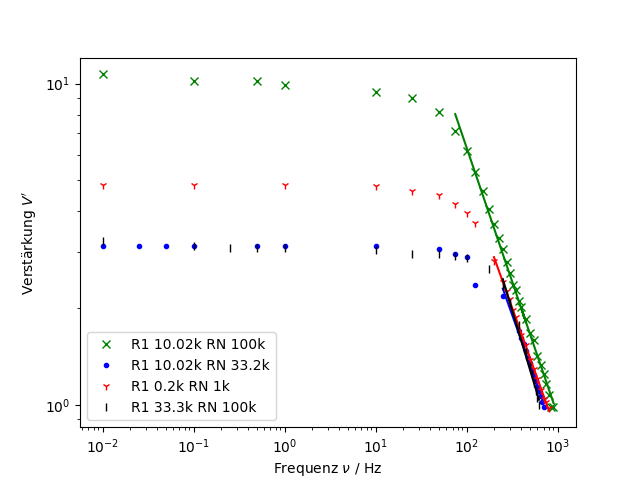
\includegraphics[width=\textwidth]{img/a.png}
	\caption{Frequenzgang eines gegengekoppelten Verstärkers - bei kleinen Frequenzen ist die Verstärkung in etwa konstant, nimmt dann aber mit größer werdenden Frequenzen exponentiell ab.}
	\label{Frequenzgang}
\end{figure}

\begin{table}
	\caption{}
	\label{}
	\begin{tabular}{ccccccc}
		$R_1/\si{\kilo\ohm}$	&	$R_\text{N}/\si{\kilo\ohm}$	&	A	&	B	&	$V^\prime$	&	$R_{N}/R_1$	&	$\nu_\text{G}/\si{hertz}$	\\
		10.02	&	100	&	-0.83\pm0.01	&	2.47\pm0.03	&	10.69 	&	9.98	&	80.74	\\
	\end{tabular}
\end{table}

\FloatBarrier
